\begin{pastexam}[label={px:ccu-115-swa-10}]{中正資工所甲組 115 學年度 第 20 題}
（複選；全對才給分）

(3\%) (\qquad) Given the fully parenthesized arithmetic expression provided below, construct the
corresponding expression tree and determine its pre-order traversal.
\begin{center}(((((A * B) -- (C * D)) -- (E / F)) + G) -- (H / I))\end{center}
(a)~-- + -- -- * A B * / C D E F G / H I \qquad (b)~-- + / -- G H I -- / * * E F A B C D\\
(c)~-- + -- -- * A B * C D / E F G / H I \qquad (d)~-- + / / G H I -- F * E -- D * C A B\\
(e)~none of the above
\end{pastexam}

\begin{pastsoln}
答案：(c)。

完全加括號的運算式，每一對括號就是一個內部節點：括號裡最外層的運算子是根，左右兩邊各是一棵
子樹（資結書第~7.7~節）。 由外往內拆：
\begin{itemize}
\item 最外層：$(\ \cdots\ ) - (H / I)$，根是 $-$，右子樹是 $H / I$。
\item 左邊 $(\ \cdots\ ) + G$：根 $+$，右子節點 $G$。
\item 再左邊 $(\ \cdots\ ) - (E / F)$：根 $-$，右子樹 $E / F$。
\item 再左邊 $(A * B) - (C * D)$：根 $-$，兩邊各是一個 $*$。
\end{itemize}
\begin{center}
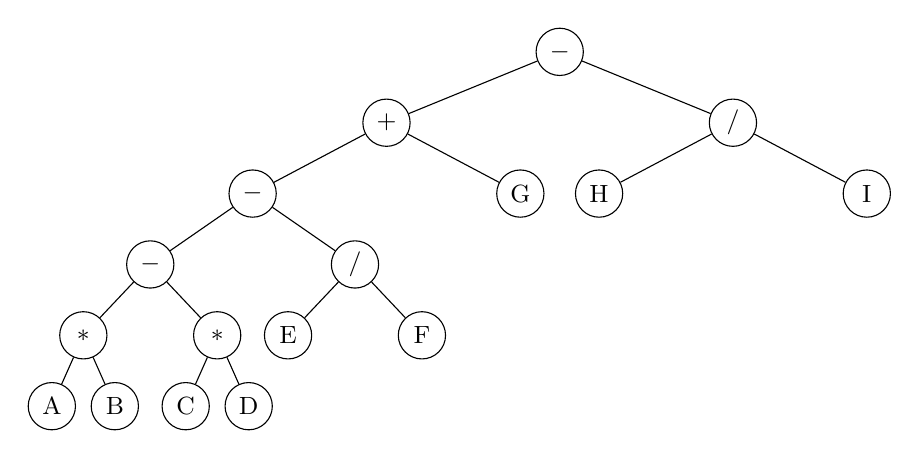
\begin{tikzpicture}[level distance=9mm,
  every node/.style={circle,draw,minimum size=6mm,inner sep=0pt,font=\small},
  level 1/.style={sibling distance=44mm},
  level 2/.style={sibling distance=34mm},
  level 3/.style={sibling distance=26mm},
  level 4/.style={sibling distance=17mm},
  level 5/.style={sibling distance=8mm}]
\node {$-$}
  child {node {$+$}
    child {node {$-$}
      child {node {$-$}
        child {node {$*$} child {node {A}} child {node {B}}}
        child {node {$*$} child {node {C}} child {node {D}}}}
      child {node {/} child {node {E}} child {node {F}}}}
    child {node {G}}}
  child {node {/} child {node {H}} child {node {I}}};
\end{tikzpicture}
\end{center}
前序（根、左、右）：$-$ $+$ $-$ $-$ $*$ A B $*$ C D / E F G / H I，就是 (c)。 檢查：把前序由右往左
掃、用堆疊求值的方式還原，每個運算子都恰好拿到兩個運算元，最後剩一棵樹，對得上。
\begin{itemize}
\item (a) 錯：前七個符號 $-$ $+$ $-$ $-$ $*$ A B 都對，接下來應該是 $*$ C D / E F，(a) 寫成
$*$ / C D E F，把 / 提到 C 前面，還原出來是 $(C / D) * E$ 之類的樹，不是題目的運算式。
\item (b)、(d) 錯：第三個符號就不合。 根 $-$、左子節點 $+$ 之後，前序的第三個是 $+$ 的左子節點
$-$，(b)、(d) 都寫成 /。
\item (e) 錯，(c) 對。
\end{itemize}
\end{pastsoln}
